
% \section{Introduction}
% \section{Main contributions}
% \section{Experiments}
% \section{Conclusion}


\section{System description}
\label{sec:system}
Grobid-quantities is a Java web application, based on Grobid (GeneRation Of BIbliographic Data)~\cite{GROBID} \cite{lopez2009grobid}, a machine learning framework for parsing and structuring raw documents such as PDF or plain text. 
Grobid-quantities is designed to process large quantity of data, via web, through a REST (Representation State Transfer) API or locally, via the file-system (batch mode). 
Output information are standardised as stand-off annotations, and they can be stored in databases or indexed in search engines. Each annotation can be visualised on top of PDFs using the GROBID build-in positional coordinates.

\subsection{Data model}
\label{subsub:data-model}
\begin{figure}[ht]
  \centering
  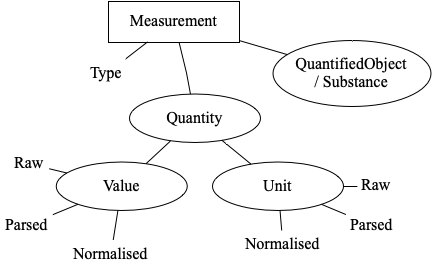
\includegraphics[width=\linewidth]{figures/quantities/schema-2.png}
  \caption{Schema of the data model.}
  \label{fig:data-model-schema-2}
\end{figure}

The data model (Figure \ref{fig:data-model-schema-2}) lay its foundation on the concept of \textit{Measurement}, which links an object or a substance with one or more \textit{quantities}. We defined four \textit{Measurements} types: (a) atomic, in case of a single measurement (e.g., 10 grams). (b) interval (\textit{from 3 to 5 km}) and (c) range ($100 \pm 4$ mm) for continuous values, and, (d) a list of discrete values. A \textit{Quantity} links the quantitative value and the unit. 
Since data extracted from PDFs unavoidably present irregular tokens from wrong UTF-8 encoding or missing fonts, we designed this model to allow partial results. The \textit{Value} and \textit{Unit} entities allow three different representations (Figure \ref{fig:data-model-schema-2}): \textit{Raw} as appear in input, \textit{Parsed} unifies the value into the numerical expression, and the unit with its properties (system, type). Finally, \textit{Normalised} contains the transformed unit and values to the SI system. \textit{Value} object supports four types of representations: numeric (2, 1000), alphabetic (two, thousand), scientific notation ($3\cdot10\textsuperscript{5}$), and time, which is also an expression of measurement. Units objects are organised following the SI, which allows representing units as products of simpler compounds (e.g. m/s to $m \cdot s\textsuperscript{-1}$) further decomposed as triples (prefix, base and power).

\subsection{Architecture}
The system takes in input text or PDF (the content is extracted in a structured way using the Grobid framework) and performs three steps: (a) tokenisation, (b) measurement extraction and parsing and (c) quantity normalisation. The details of each step are summarised as follows. 

\subsubsection{Tokenisation}
This process splits input data into tokens. Grobid-quantities uses a two-phase tokenisation: (1) first it splits by punctuation marks, then (2) each resulting token is re-tokenised to separate adjacent digits and alphanumeric characters. Given the example \texttt{25m\^{}2}, first returns a list \texttt{[25m, \^{}, 2]} and then recursively divides \texttt{25m} as \texttt{[25, m]}  resulting in \texttt{[25, m, \^{}, 2]}.

\subsubsection{Extraction}
% Quantity model 
The tokens are passed through three ML models, in cascade: first the \textit{Quantities} CRF model determines appropriate unit and value tags. Results are further processed by the respective \textit{Units} and \textit{Values} CRF models as illustrated in Figure \ref{fig:schema-cascade}.  

\begin{figure}[ht]
  \centering
  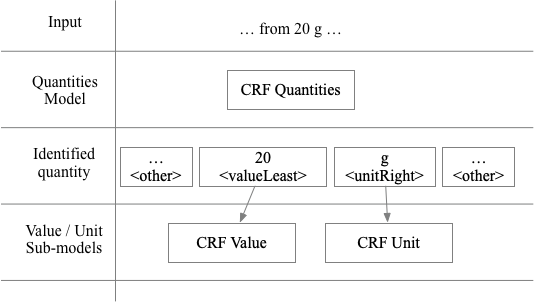
\includegraphics[width=\linewidth]{figures/quantities/schema-cascade}
  \caption{The cascade approach in applied CRF models. The Quantities model recognises value and units which are passed, respectively, to Values and Units CRF sub-models for further extraction.}
  \label{fig:schema-cascade}
\end{figure}

Table \ref{tab:quantities-model-labels} describes the labels predicted by the \textit{Quantities} CRF model. Notice that, to reconstruct complex structured objects from the flat sequence generated by the engine, additional labels are necessary (such as <unitLeft>, <unitRight>, for units).

\begin{table}[ht]
\centering
  \caption{Labels description for the Quantities CRF model. In bold are highlighted specific examples.}
  \label{tab:quantities-model-labels}
  \begin{tabular}{lll}
    \toprule
    Label & Description & Example\\
    \midrule
    valueAtomic & value of an atomic quantity & \textbf{2} m \\
    valueLeast & least value in an interval & from \textbf{2} m \\
    valueMost & max value in an interval & up to \textbf{7} m \\
    valueBase & base value in a range & $\textbf{20}\pm7$ m \\
    valueRange & range value in a range & $20 \pm \textbf{7}$ m \\
    valueList & list of quantities & \textbf{2}, \textbf{3} and \textbf{10} m \\
    unitLeft & left-attached unit & \textbf{pH} 2 \\
    unitRight & right-attached unit & 2 \textbf{m} \\
    other & everything else & - \\
  \bottomrule
\end{tabular}
\end{table}

% Gazetteers
Previous work presented extensive use of databases or ontologies. In our solution, we used a similar approach. We created a list of units (in English, French and German) with their characteristics: system (SI base, SI derived, imperial, ...) and type (volume, length, ...), and their representations: notations (m\textsuperscript{3}, \texttt{m\^{}3}), lemmas (cubic meter, cubic metre) and inflections (cubic meters, cubic metres). We made this list available through the \textit{Unit Lexicon}, which offers unit lookups by properties (such as notation, lemma, inflexion). A second gazetteer was created to allow the transformation of alphabetic values in numeric ones (for example, twenty-one to 21).

Features in the \textit{Quantities} CRF model are generated from preceding and following tokens, presence of capital, digits. Orthogonal features are obtained through the \textit{Unit Lexicon}, like a \textit{Boolean} indicating whether a token is a known unit or not. Typographical information (such as format, fonts, subscript and superscript) are ignored. 

% Unit model 
The \textit{Units} CRF model works at character level and uses the \textit{Unit Lexicon} to highlight known units or prefixes. The input tokens are parsed and transformed to a product of triples (prefix, base, power) as shown in Table \ref{tab:units-model-labels}. For example \texttt{Kg/mm\textsuperscript{2}}, corresponds to \texttt{$Kg\cdot mm\textsuperscript{-2}$} and becomes \texttt{[(K, g, 1), (m, m, -2)]} as product of triples. 

\begin{table}[ht]
\centering
  \caption{Labels description for the Units CRF model. In bold are highlighted specific examples. }
  \label{tab:units-model-labels}
  \begin{tabular}{lll}
    \toprule
    Label & Description & Example\\
    \midrule
    prefix & prefix of the unit  & \textbf{k}m\textsuperscript{2} \\
    base & unit base & k\textbf{m}\textsuperscript{2}\\
    pow & unit power & km\textsuperscript{\textbf{2}}\\
    <other> & everything else & - \\
  \bottomrule
\end{tabular}
\end{table}

We then use the structured triples to fetch the corresponding information (system, type) from the \textit{Unit Lexicon} and attach them to the resulting object. 
This implementation processes the unit characters using right-to-left order. 
%Priority modifiers, such as parenthesis, are ignored because more complex to manage and not frequent. 
Priority modifiers, such as parenthesis, are ignored. They are generally not frequent in units expressions, and require a more complex logic.

%Let's suppose the raw text contains "10 m 3". The Quantity model identifies 10 as atomic value and "m 3" as the unit. The Unit model identifies "m" as the base and "3" as power: [(,m,3)]. This product is then reformatted as "m\^3" and looked up in the gazetteer. Since "m\^3" exists, system=SI, inflection='Cubic meters' and type=volume are attached to the unit object. 
% Value model 
In parallel, the CRF \textit{Values} model unifies the format of identified values into numerical formats. It supports four types: numeric, alphabetic, scientific notation, and time expression (see Table \ref{tab:values-model-labels}). Different techniques are applied for each type: alphabetic expressions are looked up in the word-to-number gazetteer, scientific notations are parsed and calculated mathematically. Time expressions are further segmented using the Grobid built-in Date CRF model.

\begin{table}[ht]
\centering
  \caption{Labels description for the Values CRF model. In bold are highlighted specific examples.}
  \label{tab:values-model-labels}
  \begin{tabular}{lll}
    \toprule
    Label & Description & Example\\
    \midrule
    \texttt{number} & numeric value / coefficient & $\textbf{2.5}\cdot10\textsuperscript{\textbf{5}}$ \\
    \texttt{alpha} & alphabetic value & \textbf{twenty} \\
    \texttt{time} & time expression  & in \textbf{1970-01-02}\\
    \texttt{base} & base in scientific notation & $2.5\cdot\textbf{10}\textsuperscript{5}$\\
    \texttt{pow} & exponent in scientific notation & $2.5\cdot10\textsuperscript{\textbf{5}}$ \\
    \texttt{other} & everything else & - \\
  \bottomrule
\end{tabular}
\end{table}

\subsubsection{Normalisation}

The measurements extracted are transformed to the base SI unit (grams to kg, Celsius to Kelvin, etc.). We used an external Java library called Units of Measurement~\cite{units_of_measurement}, which provides a set of standard interfaces and implementations for safely handling units and quantities. Manipulating measurements with transformations often lead to common mistakes due to wrong rounding and approximations. 
At the time this paper is being written, the final revised version of this library has been accepted under the Java Standardisation Process JSR-385.

\section{Evaluation and results}
\label{sec:results}

We trained and evaluated our system's models using a dataset based on 32 scientific publications (English, Open Access (OA)) and three patents (with translation in English, French and German) randomly selected from different domains such as medicine, robotics, astronomy, and physiology. The training data was generated automatically and then corrected and cross-checked by three annotators. We used 10-fold cross-validation to evaluate each CRF model, independently, and produce precision, recall and f1 scores, as summarised in Table \ref{tab:quantities-evaluation}. 

\begin{table}[ht]
    \centering
   \caption{Summary of the evaluation scores (precision, recall, F1-score) and label contribution (support) for \textit{Quantities}, \textit{Units} and \textit{Values} CRF models, respectively. }
   \label{tab:quantities-evaluation}
   \begin{tabular}{c|cccc}
        \toprule
        Label & Precision & Recall & F1 & Support\\
        \toprule
        \multicolumn{5}{c}{\textbf{Quantities CRF model}}\\
        \midrule
        \texttt{unitLeft}          & 96.76 & 94.71 & 95.71 & 2805  \\
        \texttt{unitRight}         & 93.06 & 72.1  & 80.02 & 120   \\
        \texttt{valueAtomic}       & 85    & 84.77 & 84.84 & 3599  \\
        \texttt{valueBase}         & 78.82 & 76.52 & 77.53 & 94    \\
        \texttt{valueLeast}        & 85.05 & 77.39 & 80.94 & 862   \\
        \texttt{valueList}         & 72.09 & 54.87 & 61.33 & 494   \\
        \texttt{valueMost}         & 84.09 & 73.03 & 78.07 & 878   \\
        \texttt{valueRange}        & 84.56 & 81.5  & 82.68 & 93    \\
        all (macro avg.)    & 84.93 & 76.86 & \textbf{80.14}\\
        \midrule
        \multicolumn{5}{c}{\textbf{Unit CRF model}}\\
        \midrule
        \texttt{base}              & 99.02 & 99.22 & 99.12 & 3075      \\
        \texttt{pow}               & 98.04 & 98.9  & 98.46 & 322       \\
        \texttt{prefix}            & 99.19 & 98.8  & 98.99 & 821       \\
        all (macro avg.)    & 98.75 & 98.97 & \textbf{98.86}    \\
        \midrule
        \multicolumn{5}{c}{\textbf{Values CRF model}}\\
        \midrule
        \texttt{alpha}             & 96.64  & 98.65 & 97.62  & 826      \\
        \texttt{base}              & 83.06  & 69.23 & 72.77  & 58       \\
        \texttt{number}            & 98.01  & 99.02 & 98.52  & 3858     \\
        \texttt{pow}               & 76.45  & 74.67 & 74.58  & 56       \\
        \texttt{time}              & 72.54  & 87.83 & 79.34  & 322      \\
        all (macro avg.)    & 85.34  & 85.88 & \textbf{84.57} & -\\
        \bottomrule
   \end{tabular}
\end{table}

% Scores + discussion Quantities CRF model 
The Quantities CRF model reported an f1 macro average of 80.14\% with precision and recall of 84.93\% and 76.86\%, respectively. The paragraph accuracy was 68.97\%, indicating that more than half of the evaluated paragraphs were correctly labelled. These scores are promising, considering the complexity of the task and the rather small size of the training corpus. In particular, \texttt{<list>} and \texttt{<unitRight>} require more example. 

% Scores + discussion Unit CRF model 
The Units CRF model f1 macro average was 98.86\%, with precision and recall reaching 98.75\% and 98.97\%, respectively. Compared with our other models, performances were extremely high (more than 10\% for f1 score). 
Such difference can be attributed to the data distribution and the lower variability of unit expressions. We analysed the training data, and we noticed that the distribution is biased toward simple units (composed by a single triple). Intuitively, this makes sense, because simple units are statistically more frequent; on the other hand, it highlights the necessity of having more complex examples in our dataset. 
Secondly, unit expressions appear, by nature, with lower variability, leading to the generation of more duplicates than in other models' training datasets. For example, the expressions 1\% and 2\% have two different values (1, 2) and the same unit (\%), which would appear twice. 
Since we cannot alter the statistical distribution of the dataset, we would obtain better and more precise measurements of the model generalisation capabilities by using a separate and independent evaluation corpus. 

% Scores + discussion Values CRF model 
The Value CRF model scored average macro f1 at 85.64\% with precision and recall at 81.82\% and 93.29\%, respectively.
We noticed that both \textit{<base>}, \textit{<pow>} and \textit{<time>} have lower f1-score. While \textit{<base>} and \textit{<pow>} require more training data, \textit{<time>} expressions may overlap with \textit{<number>} suggesting more contextual information should be introduced. 


\section{Applications}
\label{sec:use_cases}
Recently, the normalised data extraction is strongly required in materials research. The inverse problem in which high-performance materials are predicted from properties is expected to be solved with well-organised big data. At the National Institute for Materials Science (NIMS), a project to discover new superconducting materials from scientific literature is in progress. The system being developed relies on Grobid-quantities to extract and normalise superconducting properties, such as critical temperature (Tc) with units of mK and K and critical pressure expressed with units of Pa, MPa, and GPa \cite{foppiano2019proposal}. 

Grobid-quantities was showcased in a Text and Data Mining (TDM) platform (within the scope of the French national-wide ISTEX~\cite{dazy2014istex} project) where it provided measurement annotations used to prototype a quantities-based semantic search\footnote{The demo can be accessed at \url{https://traces1.inria.fr/istex_sample/}}. 

Finally, another use was made in a system for extracting semantic measurements and meaning in Earth Science, Marve~\cite{hundman2017measurement}.  